%************************************************
\chapter{The Simulation}
\label{chapter:the_simulation}
%************************************************

My description of the model of mind in plain non-technical English is
now complete.  The rest of this dissertation will extend the model
that I have completed describing in English into the assumptions of
simulation that I will need for the mathematical evaluation in this
part.

There is a difference between a model of mind and a simulation of a
model of mind.  I have presented my model of mind in plain English in
the first part of this dissertation.  Simulating the model does not
change the model.  At this point, I am assuming that I have
communicated my model of mind.  I will now augment this model with an
understanding of how to simulate it.  It is important to explain how
the model can be simulated, so that I can subsequently quantify
metrics for evaluation.  Further, understanding how to simulate the
model is imperative to understanding the computational implementation.

\section{Simulation Model}

I will use the term \emph{simulation model} to refer to the model that
changes during the dynamic activity of \emph{simulation}.  Because a
model is a static arrangement of symbols, these changes are
necessarily discrete.  It is imperative to understand that the
simulation model is not the same as the model that I have previously
described.  The model of mind does not change in this dissertation.
The simulation model is an arrangement of symbols that can be
manipulated, simulating the model of mind.  The simulation model is
meant to change as the simulation proceeds.  I use the term simulation
as a general reference to the dynamic activity in Duration that
manipulates the simulation model.  Thus, when I describe the
simulation model, I will be careful to not give a definition of the
dynamic activity of simulation itself in terms of a static model.  The
term simulation will be the only reference to activities in Duration
that I will make as I describe the simulation model.  This is
necessary if this model of simulation is to be used to simulate
anything.  Thus, I will not define the term simulation in terms of
other symbols, this term can be given any subsequent grounding that
would focus on a simulation model of something specific.

The simulation model explicitly represents the changing aspects of the
model of mind as a model itself.  I have carefully left the activities
in my model of mind as the undescribed dynamic referent of a symbol.
The activities in my model are prior to their symbolization, so
assumptions are necessary for referring to these activities
symbolically in the simulation model.  Each assumption made in
symbolizing the ongoing activities in Duration restricts the
simulation model from being a model of those assumptions.

For example, the first assumption I will make of the simulation model
is that the activities in Duration are discrete and that they can be
represented by a mathematical set of symbols.  This is a critical
assumption that I have purposefully avoided until now.

\section{Static Sets of Dynamic Activities}

\begin{figure}[bth]
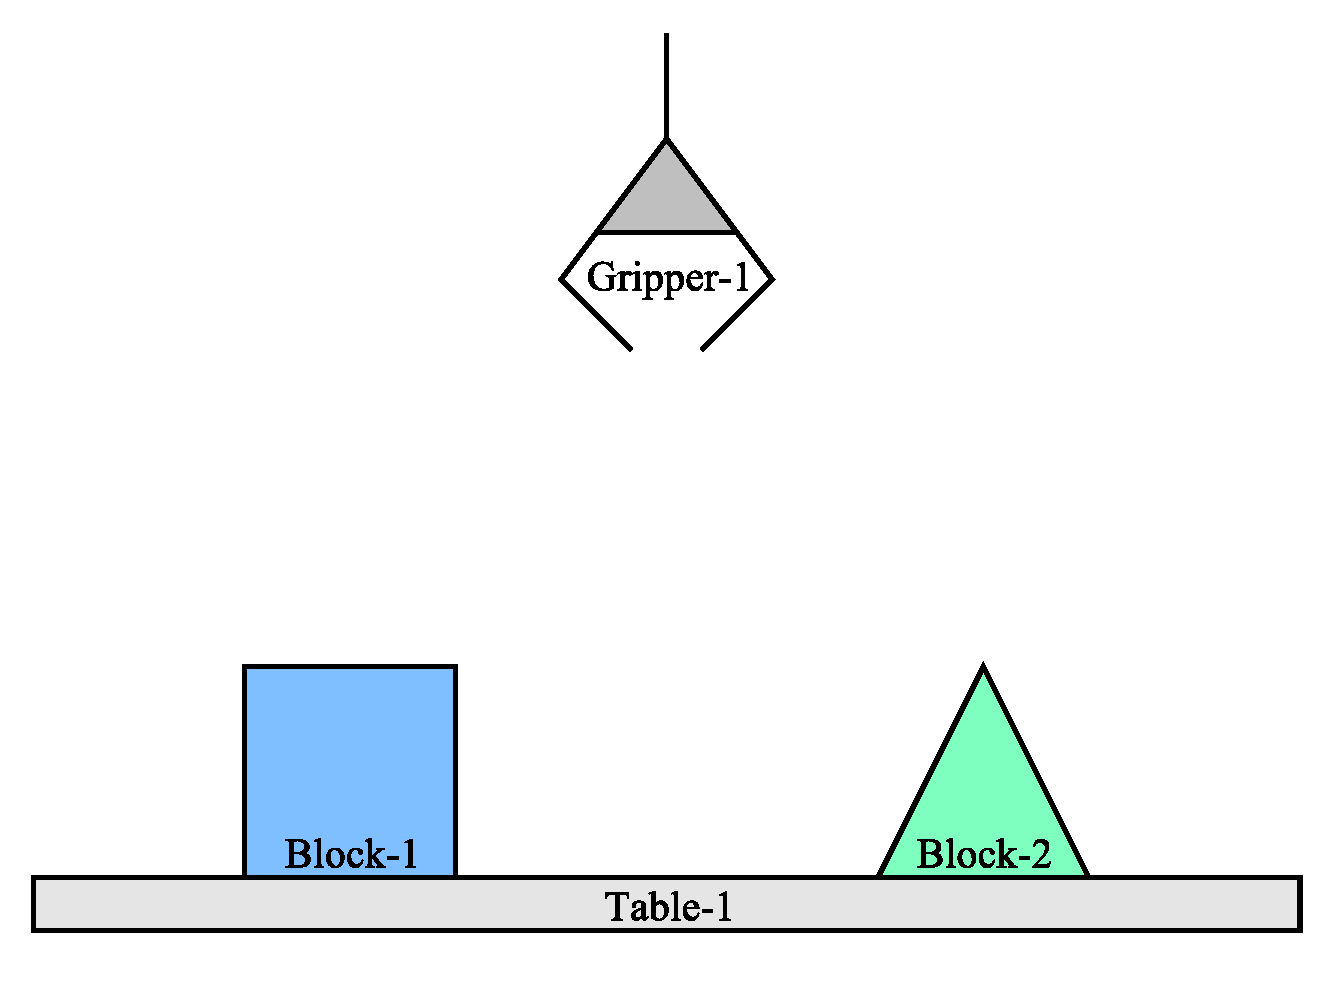
\includegraphics[width=10cm]{gfx/blocks_world_simulation}
\caption{An example for simulation.}
\label{figure:blocks_world_simulation}
\end{figure}

I will begin with a relatively simple model of the activities in
Duration in order to describe my model of simulation.  One of the
simplest mathematical models is a \emph{set} of symbols.  I will first
describe the simulation model as the mathematical set, $S$,
the state.  Here is an example of a possible symbolization of the
activities shown in \autoref{figure:blocks_world_simulation}:
\begin{equation}
\label{equation:example_initial_state}
S =
  \left\{
    \begin{array}{l}
      \text{{\tt Block-1-sitting-on-Table-1}}, \\
      \text{{\tt Block-2-sitting-on-Table-1}}, \\
      \text{{\tt Block-1-sitting-on-Table-1}}, \\
      \text{{\tt Gripper-1-being-above-Table-1}}, \\
      \text{{\tt Gripper-1-moving-left}}
    \end{array}
  \right\}
\end{equation}

During the simulation, the state, $S$, changes.  The
simulation process is a discrete stepwise activity that results in
different symbols being contained in the state set, $S$.  I
will now describe a notation for referring to the different states
that result from a simulation process.

\section{Simulation States}

Equations~\ref{equation:simulate_first}
and~\ref{equation:simulate_last} show a notation for referring to the
state of a simulation after a number of simulation steps, $n$.
\begin{align}
\label{equation:simulate_first}
S[0] &= \text{\emph{The Initial State}} \\
\label{equation:simulate_last}
S[n] &= \text{simulate}~S[n-1]
\end{align}
Equation~\ref{equation:simulate_first} defines $S[0]$ to be
the initial representation of the activities in Duration that are
being simulated; an example of the initial state was given previously
in Equation~\ref{equation:example_initial_state}.
Equation~\ref{equation:simulate_last} introduces an explicit reference
to the activity of simulation with the symbol ``simulate.''  Because I
have not yet defined this activity, these equations still have a
reference to the actual dynamic activity of simulation.  I use this
notation to discuss how the state, $S$, changes during the
actual process of simulation.  I will use the notation in
Equation~\ref{equation:simulate_n_steps} to refer to the state of the
simulation after $n$ actual steps of simulation activity:
\begin{equation}
\label{equation:simulate_n_steps}
S[n] = \text{simulate}^n~S[0]
\end{equation}

\section{State Transitions}

\autoref{figure:blocks_world_gripper_over_block} shows an example of
the next state of the simulation, $S[1]$.
Equation~\ref{equation:example_next_state} gives an example
description of the next state of the simulation model:
\begin{figure}[bth]
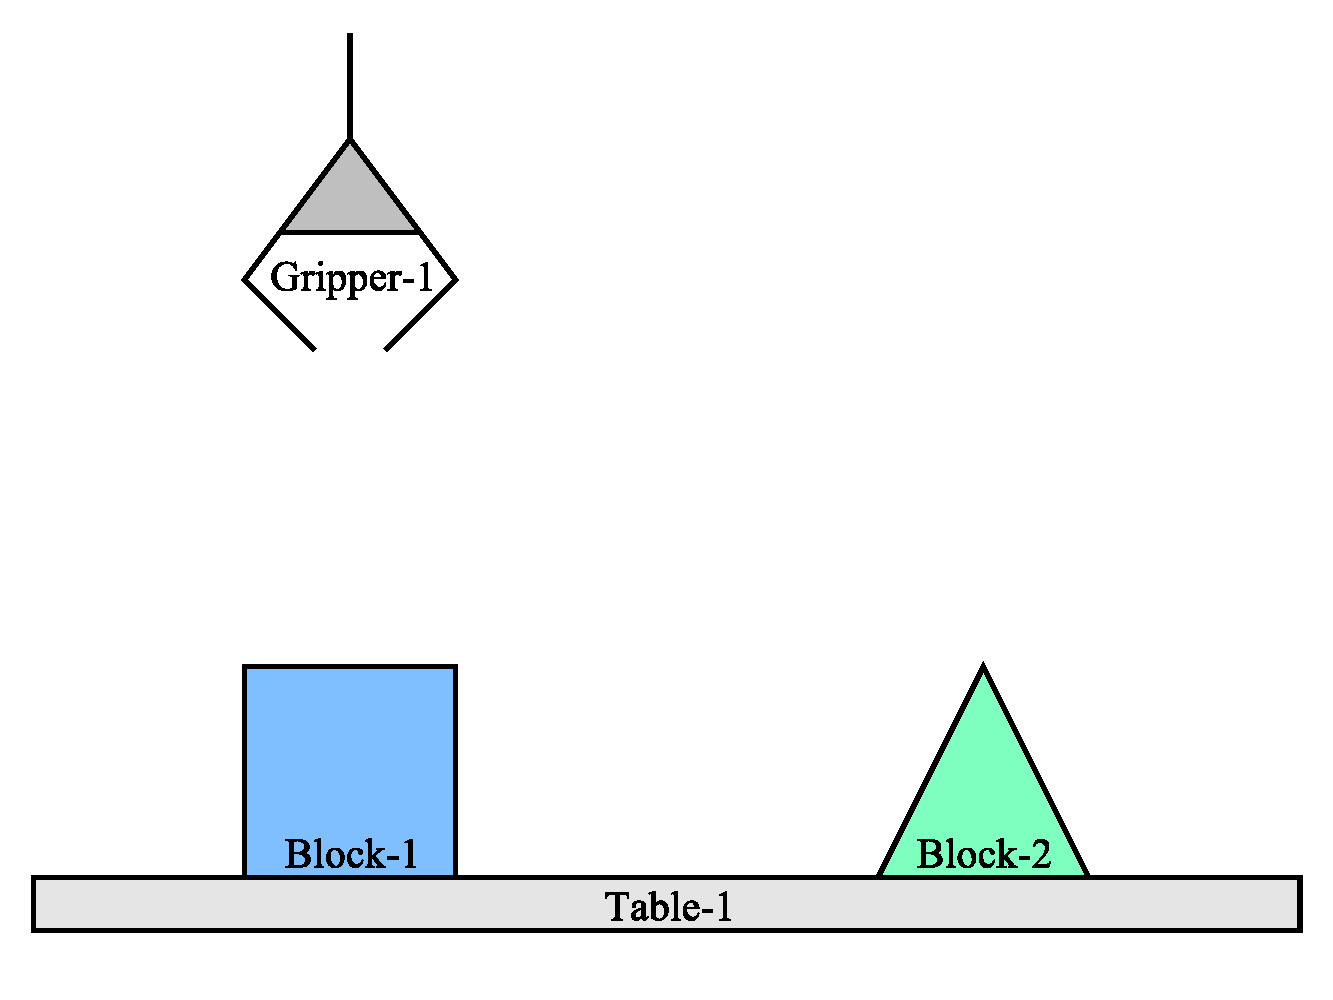
\includegraphics[width=10cm]{gfx/blocks_world_gripper_over_block}
\caption{An example future state of simulation.}
\label{figure:blocks_world_gripper_over_block}
\end{figure}
\begin{equation}
\label{equation:example_next_state}
S[1] =
  \left\{
    \begin{array}{l}
      \text{{\tt Block-1-sitting-on-Table-1}}, \\
      \text{{\tt Block-2-sitting-on-Table-1}}, \\
      \text{{\tt Gripper-1-hovering-above-Table-1}}, \\
      \text{{\tt Gripper-1-hovering-above-Block-1}}
    \end{array}
  \right\}
\end{equation}

Now, in order to begin to describe the activity of simulation, we must
explicitly represent the transition, $T$, from one state to another.
I refer to the resulting change to the state of the simulation as a
\emph{state transition}.  The transition, $T[n]$, consists of two sets
that keep track of changes, the \emph{add} set and the \emph{remove}
set, as shown in Equation~\ref{equation:state_transition}:
\begin{equation}
\label{equation:state_transition}
T[n] = \{T_\text{add}[n], ~T_\text{remove}[n]\}
\end{equation}
Equations~\ref{equation:predictive_state_transition}
through~\ref{equation:transframe_last} give a definition of the
transition, $T[n]$, in terms of the states, $S[n]$ and
$S[n+1]$:
\begin{align}
\label{equation:predictive_state_transition}
          S[n+1] & = S[n] ~{\cup}~ T_\text{add}[n] ~{\setminus}~ T_\text{remove}[n] \\
         T_\text{remove}[n] & ~{\subseteq}~ S[n] \\
         T_\text{remove}[n] & ~{\not\subseteq}~ S[n+1] \\
            T_\text{add}[n] & ~{\subseteq}~ S[n+1] \\
\label{equation:transframe_last}
            T_\text{add}[n] & ~{\not\subseteq}~ S[n]
\end{align}
Equations~\ref{equation:state_transition_first}
and~\ref{equation:state_transition_last} give the state transition,
$T[n]$, for every step of the simulation:
\begin{align}
  \label{equation:state_transition_first}
     T_\text{add}[n] &= S[n+1] ~{\setminus}~ S[n] \\
  \label{equation:state_transition_last}
  T_\text{remove}[n] &= S[n]   ~{\setminus}~ S[n+1]
\end{align}
Equation~\ref{equation:predictive_state_transition} shows the
predictive potential for knowing the transition, $T[n]$, given the
current state, $S[n]$.  Of course, $T[n]$ is defined in
terms of $S[n]$ \emph{and} $S[n+1]$, so any
predictive potential for
Equation~\ref{equation:predictive_state_transition} is purely
hypothetical.

\section{Symbols and Simulated Symbols}

It becomes important at this point to keep track of the layer of
modelling that results when one simulates thinking.  Therefore, I will
use an asterisk notation for referring to different classes of
simulated modelling.  For example, I will continue to use, simply, the
term symbol to refer to the symbols that have actually been
reflectively symbolized in order to refer to the activities in
Duration.  The set of symbols that refer to dynamic activities in
Duration are defined in Equation~\ref{equation:everything_symbolized}
to be $\mathcal{S}[n]$, the union of all states in the simulation
state from $S[0]$ to $S[n]$:
\begin{equation}
\label{equation:everything_symbolized}
\mathcal{S}[n] = \bigcup_{k=0}^n{S[k]}
\end{equation}
When I am referring to the simulation of the process of symbolization,
I will refer to this as a simulated symbol, or a \emph{symbol*}.  A
symbol* is a simulated symbol that is created by the simulation.  The
symbol* is a static reference that is simulated as being grounded in
the symbols in the simulation state, the simulated activities in
Duration.

\section{Representing Existence}

Activities actually exist.  Once we have considered the activities in
Duration to be the set of symbols, $S$, we have assumed static
representations for the actual dynamic.  The dynamic does not have
terms to help us in representing, so we use the static Spatial
arrangement, time.  Therefore, the question of existence becomes a
question of whether or not a symbol is in specific ordered position of
a static Spatial arrangement.  Equation~\ref{equation:exists} shows a
definition of {\tt exists}, a logical relationship between any
symbolic reference to activity contained in the simulation present or
previously:
\begin{equation}
\label{equation:exists}
\text{exists}(x, n) = x{\in}S[n], \text{ for all }x{\in}\mathcal{S}[n]
\end{equation}

\section{Representing Symbolization}

In order to describe symbolization, a representation for a simulated
symbol must be defined.  A simulated symbol is actively maintained in
Duration, so the existence of a simulated symbol in the simulation
model would need to be added to the set of all simulated activities in
Duration.  The symbol*, $x^*$, has a referent,
$\text{referent}(x^*,~n)$, a subset of the previous simulated
activities in Duration, $\mathcal{S}[n-1]$, in
Equations~\ref{equation:symbolization_first}
and~\ref{equation:symbolization_last}:
\begin{align}
\label{equation:symbolization_first}
                    x^* &= \text{\emph{Simulated Symbol}} \\
\label{equation:symbolization_last}
\text{referent}(x^*, n) &\subseteq \mathcal{S}[n-1]
\end{align}
Equation~\ref{equation:existence_of_symbol} defines the relationship
between the existence of a simulated symbol, $\text{exists}(x^*, n)$,
the simulation state, $S[n]$, and the simulated referent,
$\text{referent}(x^*, n)$.  This equation shows that if any symbol
that is contained within the simulated referent set is in the
simulation state, the symbol* exists:
\begin{equation}
\label{equation:existence_of_symbol}
(S[n] ~{\cap}~ \text{referent}(x^*, n)) \neq \emptyset ~\longleftrightarrow~ \text{exists}(x^*, n)
\end{equation}

\section{Tautological Symbolic Reference}

Consider the following definition, which defines a symbol* to
tautologically reference its own symbolization activity.
Equation~\ref{equation:tautological_reference} defines a tautological
referent for a symbol*, $x^*$:
\begin{equation}
\label{equation:tautological_reference}
x^* \in \text{referent}(x^*, n)
\end{equation}
Equations~\ref{equation:tautological_derivation_first}
through~\ref{equation:tautological_derivation_last} derive how
Equation~\ref{equation:tautological_reference} leads to a tautology,
removing the utility from the entire system of equations that define a
symbol*.  Equation~\ref{equation:tautological_derivation_first}
derives from a combination of the existence equation,
Equation~\ref{equation:existence_of_symbol}, and the tautology
equation, Equation~\ref{equation:tautological_reference}:
\begin{align}
\label{equation:tautological_derivation_first}
%(S[n] ~{\cap}~ \text{referent}(x^*, n)) \neq \emptyset ~&\longleftrightarrow~ \text{exists}(x^*, n) \\
                                          x^* \in S[n] ~&\longleftrightarrow~ \text{exists}(x^*, n) \\
                                          x^* \in S[n] ~&\longleftrightarrow~ [(S[n] ~{\cap}~ \text{referent}(x^*, n)) \neq \emptyset] \\
                                          x^* \in S[n] ~&\longleftrightarrow~ x^* \in S[n] \\
\label{equation:tautological_derivation_last}
                                                       ~&\text{\emph{True}}
\end{align}

Because a tautological reference, like that in
Equation~\ref{equation:tautological_reference}, removes all utility
from symbols* in the simulation model, it is important that
tautological references are avoided.  In order to avoid tautological
references, I define an ordering for symbolic references that keeps
references from ever becoming purely tautological.

\section{Sets of Symbol Activities}

Symbols are the static counterpart to the dynamic in the model of
mind.  Keeping track of which activities are dynamic and which are
static and symbolic is critical for avoiding the creation of a
tautological model with symbols only referring to other symbols.
Equations~\ref{equation:symbol_activities_set_first}
and~\ref{equation:symbol_activities_set_last} define the set of
activities that are symbolic references:
\begin{align}
\label{equation:symbol_activities_set_first}
X^*_i &= \text{\emph{Symbol activities in reflective}}^i\text{\emph{ layer}} \\
\label{equation:symbol_activities_set_last}
X^*_i &\subseteq L_i
\end{align}

\section{Layers of Sets of Dynamic Activity}

In order to avoid tautological symbolic references, I have divided the
model into layers that order symbolic activities and references.  To
simulate the $\text{reflective}^n$ layers of activity in the model, I
must divide the simulation state, $S$, into reflective layers.
Equations~\ref{equation:layers_of_sets_first}
through~\ref{equation:layers_of_sets_last} give a definition of the
disjoint set of layers, $\mathbf{L}$, stating that the union of all
layers of activity is equal to the simulation state, $S$:
\begin{align}
\label{equation:layers_of_sets_first}
                            L_i &= \text{\emph{Activities of the} }\text{reflective}^i\text{ \emph{layer}} \\
                     \mathbf{L} &= \{L_0, ~L_1, ~L_2, ~...~ \} \\
\forall_{A,B{\in}{\mathbf{L}}} ~ (A &= B ~{\vee}~ A{\cup}B = {\emptyset}) \\
\label{equation:layers_of_sets_last}
                      S &= \bigcup_{A{\in}\mathbf{L}}{A}
\end{align}

Using these reflective layer definitions, I define an ordering of
symbol* references that prevents symbols from every having
tautological references.
Equation~\ref{equation:layered_symbol_references} defines that a
symbol may only refer to activities in the layers below its own layer
of activity:
\begin{equation}
\label{equation:layered_symbol_references}
x^* \in L_i \rightarrow \text{referent}(x^*, n) \subseteq \bigcup_{k=0}^{i-1}{L_k}
\end{equation}

\section{No Symbols* in Layer Zero}

Equations~\ref{equation:no_symbols_in_layer_zero_first}
through~\ref{equation:no_symbols_in_layer_zero_last} derive that a
symbol* cannot actively exist in the simulated reflective layer zero,
$L_0$.  Equation~\ref{equation:no_symbols_in_layer_zero_first} derives
from the layered symbolic references equation,
Equation~\ref{equation:layered_symbol_references}.
Equation~\ref{equation:no_symbols_in_layer_zero_exists} derives from
incorporating a reversed version of the symbol existence equation,
Equation~\ref{equation:existence_of_symbol}:
\begin{align}
\label{equation:no_symbols_in_layer_zero_first}
       x^* \in L_0 \rightarrow \text{referent}(x^*, n) &\subseteq \emptyset \\
\text{\emph{True}} \rightarrow \text{referent}(x^*, n) &= \emptyset \\
                               \text{referent}(x^*, n) &= \emptyset \\
\label{equation:no_symbols_in_layer_zero_exists}
\text{exists}(x^*, n) &\longleftrightarrow (S[n] ~{\cap}~ \emptyset) \neq \emptyset \\
\text{exists}(x^*, n) &\longleftrightarrow \emptyset \neq \emptyset \\
\text{exists}(x^*, n) &\longleftrightarrow \text{\emph{False}}
\label{equation:no_symbols_in_layer_zero_last}
\end{align}

\section{Simulating Space}

The activity of maintaining a Spatial relationship, $r_i$, occurs in
the $\text{reflective}^i$ layer.
Equations~\ref{equation:define_space_activity_first}
through~\ref{equation:define_space_activity_right} define how symbols
are Spatially arranged, $r_i$, from the layer below:
\begin{align}
\label{equation:define_space_activity_first}
              r_i &= \text{\emph{Spatial relationship activity in} reflective}^i\text{\emph{ layer}} \\
              r_i &\in L_i \\
\label{equation:define_space_activity_left}
 \text{left}(r_i) &\in X^*_{i+1} \\
\label{equation:define_space_activity_right}
\text{right}(r_i) &\in X^*_{i+1}
\end{align}
Equations~\ref{equation:define_space_activity_left}
and~\ref{equation:define_space_activity_right} define the {\tt left}
and {\tt right} symbolic referents of the $r_i$ simulated Spatial
relationship.  Note that the simulated Spatial arrangement activity is
in the layer below the symbols* that are being arranged.

Spatial relationships can refer to other Spatial relationships from
the same layer because the activity of the Spatial relationship is in
the layer below the symbols that it arranges, so one arrangement can
be symbolized and referred to by another arrangement from the same
layer.

The {\tt left} and {\tt right} symbolic* referents of the simulated
relationship are modelled after the ``cons'' cell of a Lisp program.
A two-part relationship that can be symbolized and put into other
two-part relationships is enough representation to write the entire
Lisp programming language.  So, the simulated relationship, $r_i$,
allows for representing any computer science object.

\section{Simulating the Transition}

Equations~\ref{equation:define_transition_activity_first}
through~\ref{equation:define_transition_activity_future} define a
transition, $t_i$:
\begin{align}
\label{equation:define_transition_activity_first}
               t_i &= \text{\emph{Transition activity in the} reflective}^i\text{\emph{ layer}} \\
               t_i &\in L_i \\
\label{equation:define_transition_activity_past}
  \text{past}(t_i) &\in X^*_{i+1} \\
\label{equation:define_transition_activity_future}
\text{future}(t_i) &\in X^*_{i+1}
\end{align}

\section{Simulating the Hypothesis}

Equations~\ref{equation:define_hypothesis_activity_first}
through~\ref{equation:define_hypothesis_activity_result} define a
hypothesis, $h_i$:
\begin{align}
\label{equation:define_hypothesis_activity_first}
                  h_i &= \text{\emph{Hypothesis activity in the} reflective}^i\text{\emph{ layer}} \\
                  h_i &\in L_i \\
\label{equation:define_hypothesis_activity_cause}
    \text{cause}(h_i) &\in X^*_{i+1} \\
\label{equation:define_hypothesis_activity_necessity}
\text{necessity}(h_i) &\in X^*_{i+1} \\
\label{equation:define_hypothesis_activity_result}
   \text{result}(h_i) &\in X^*_{i+1}
\end{align}

\section{Simulating the Plan}

Equations~\ref{equation:define_hypothesis_activity_first}
through~\ref{equation:define_hypothesis_activity_result} define a
hypothesis, $h_i$:
\begin{align}
\label{equation:define_hypothesis_activity_first}
                  h_i &= \text{\emph{Hypothesis activity in the} reflective}^i\text{\emph{ layer}} \\
                  h_i &\in L_i \\
\label{equation:define_hypothesis_activity_cause}
    \text{cause}(h_i) &\in X^*_{i+1} \\
\label{equation:define_hypothesis_activity_necessity}
\text{necessity}(h_i) &\in X^*_{i+1} \\
\label{equation:define_hypothesis_activity_result}
   \text{result}(h_i) &\in X^*_{i+1}
\end{align}

